\documentclass[conference]{IEEEtran}
%\IEEEoverridecommandlockouts
% The preceding line is only needed to identify funding in the first footnote. If that is unneeded, please comment it out.
\usepackage{amsmath,amssymb,amsfonts}
%\usepackage{algorithmic}
\usepackage{graphicx}
\usepackage{textcomp}
\usepackage{xcolor}
\usepackage{float}
\usepackage{cite}
\usepackage{url}
\def\BibTeX{{\rm B\kern-.05em{\sc i\kern-.025em b}\kern-.08em
    T\kern-.1667em\lower.7ex\hbox{E}\kern-.125emX}}
\begin{document}

\title{Sensors Lab Conference}

\author{\IEEEauthorblockN{Gabriele Paris}
\IEEEauthorblockA{\textit{Dept physic} \\
\textit{University of Antwerp}\\
Antwerp, Belgium \\
gabriele.paris@student.uantwerpen.be}
\and
% Cut out 3rd author block as Miroslav is not contributing.
\IEEEauthorblockN{Pieter Hendriks}
\IEEEauthorblockA{\textit{Dept computer science} \\
\textit{University of Antwerp}\\
Antwerp, Belgium \\
pieter.hendriks@student.uantwerpen.be}
}

\maketitle

\begin{abstract}
In this paper, we assess the energy performance of TSCH and 6TiSCH using the Contiki-NG operating system on Zolertia RE-mote (Rev. B) nodes.\\
These boards are part of the IoT hardware family, and they allow for the creation of a network minimizing energy consumption.\\
The paper is subdivided into three main sections: in the first one, we will compare the energy consumption of the leaf and root node (LLC) at first using up to the MAC TSCH layer, and then using the full stack.\\
In the second section, we will analyze the TSCH joining process and relative energy consumption. Further, in the final section, we will assess the performance of the TSCH mode over various distances.
\end{abstract}

\begin{IEEEkeywords}
6TiSCH, Contiki-NG, Energest, IEEE 802.15.4, Power Consumption, Range, Time Slotted Channel Hopping, TiSCH, TSCH, Zolertia
\end{IEEEkeywords}

\section{Introduction}
The IETF IPv6 over the TSCH mode of IEEE802.15.4e (6TiSCH) working group has standardized a set of protocols to enable low power industrial-grade IPv6 networks. 6TiSCH proposes a protocol stack rooted in the Time Slotted Channel Hopping (TSCH) mode of the IEEE802.15.4-2015 standard, supports multi-hop topologies with the IPv6 Routing Protocol for Low-Power and Lossy Networks (RPL) routing protocol, and is IPv6-ready through 6LoWPAN\cite{6tischDef}.

Contiki-NG is an operating system for resource-constrained devices in the Internet of Things. Contiki-NG contains an RFC-compliant, low-power IPv6 communication stack, enabling Internet connectivity. The system runs on a variety of platforms based on energy-efficient architectures such as the ARM Cortex-M3/M4 and the Texas Instruments MSP430. The code footprint is on the order of a 100 kB, and the memory usage can be configured to be as low as 10 kB. 

This paper serves as an initial look at the performance of TSCH on the Contiki-NG operating system. Specifically, we look at the energy consumption by the TSCH network stack vs the 6TiSCH network stack, we analyze the TSCH joining process, and we measure the impact node separation has on the network's performance and energy characteristics.

The hardware in use are Zolertia RE-Mote boards, designed jointly with universities and industry partners in RERUM European project, to ease the development of private and secure applications for IoT and Smart City applications.\\
The RE-Mote packs several onboard resources, like an RTC, external WDT, Micro-SD, RF switch, and a Shutdown mode to reduce its power consumption down to 150nA\cite{contiki-NGWiki}.

\section{Related Work}
\subsection{Accurate energy consumption using Energest}
In section \ref{section:task1} of this paper, we focus on the analysis of the energy consumption between leaf and root node. This analysis can be done by knowing different parameters like current, tension, and time.\\
tension is always $3.3V$, current instead should be correctly provided in the board datasheet, previous works have shown that real current consumption values are different from the datasheet provided ones\cite{EnergyConsumption}, in this paper, we are going to use such current measurements to determine the energy consumption.
\subsection{Throughput Analysis} In this paper, an analysis of the throughput performance of TSCH networks is made. They show which parameters of the TSCH networks (node count, hop count, ...) influence the throughput metric in what way. Our research focuses on different performance characteristics of the TSCH implementation and can be useful alongside these results\cite{ThroughputEvaluation}. 

\section{Analysing the 6TiSCH energy consumption}
\label{section:task1}
In the first analysis, we compared the energy consumption during a certain time period of the entire 6TiSCH stack to when only enabling the TSCH MAC layer (without link-layer security) after network convergence.\\
The full stack can be seen as in Figure \ref{fig:6tischStack}.


For both analyses, we report on the consumption of the root and the leaf node separately.\\
Following we remark differences in energy consumption between the root and the leaf node in the two different scenarios.

The Time-Slotted Channel Hopping (TSCH) mode for medium access control (MAC) included in the standard IEEE 802.15.4 has been designed as the multichannel MAC protocol for Low-power and lossy networks (LLNs), a key component of the Internet of Things (IoT). Its flexibility makes the TSCH mode a very promising candidate for the future of the MAC layer in LLNs. As such, its performance under different conditions must be assessed, so that accurate guidelines for its application can be drawn\cite{TSCHExperimentEval}.
\begin{figure}[]
	\centering
	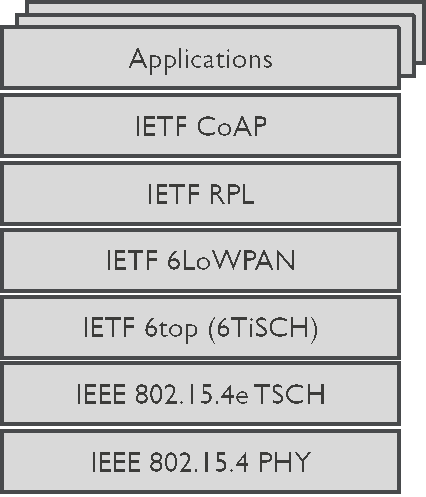
\includegraphics[width=.25\textwidth,keepaspectratio]{6TiSCH-Protocol-Stack.png}
	\caption{6TiSCH Protocol Stack\cite{TimeCritical6tisch}.}
	\label{fig:6tischStack}
\end{figure}


the physical setup of the experiment consists of two Zolertia  Remote RevB boards placed at a fixed distance of approximately 20 cm as shown in Figure \ref{fig:exp1Topology}.
\begin{figure}[H]
	\centering
	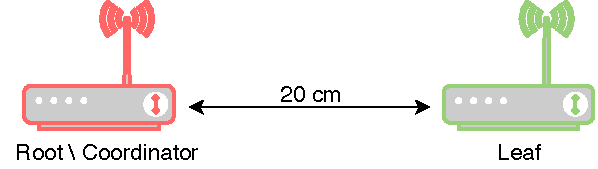
\includegraphics[width=.35\textwidth,keepaspectratio]{exp1Topology.pdf}
	\caption{Network topology for 6TiSCH energy consumption analysis.}
	\label{fig:exp1Topology}
\end{figure}
The basic setup for the following analysis are a root (coordinator) node and a leaf node that exchange the same ammount of data packets.\\
Both nodes are configured to measure the energy consumption by the Energest\footnote{https://github.com/contiki-ng/contiki-ng/wiki/Documentation:-Energest} module available in Contiki-ng\footnote{https://github.com/contiki-ng}.\\
The Energest module can be used to implement lightweight, software-based energy estimation approach for resource-constrained IoT devices. By tracking the time various hardware states such as the radio is turned on, and by knowing the power consumption of the state, it is possible to estimate the energy consumption\cite{contiki-NGWiki}.\\
The energy consumption is measured referring to the following formula:
\begin{equation}
	E_{tot}=\sum_{s \in state}^{N_{s}}E_{s}=\sum_{s \in state}^{N_{s}}I_s  \cdot V_{cc} \cdot t
\end{equation}
Where $V_{cc}$ is the supply voltage, fixed as a constant at the value $3.3V$, $I_s$ is provided by the Table \ref{tab:CurrentConsumption} column \textit{Device profiling}\cite{EnergyConsumption}, and $t$ is measured using Energest.\\
All measurements are performed in a span of 15 minutes each.
\begin{table}[htbp]
	\begin{center}
		\begin{tabular}{ccc}
			\hline
			\textbf{State}    & \textbf{\begin{tabular}[c]{@{}c@{}}CC2538\\ datasheet\end{tabular}} & \textbf{\begin{tabular}[c]{@{}c@{}}Device\\ profiling\end{tabular}} \\ \hline
			\textbf{CPU}      & 20 mA                                                               & 15.35mA                                                             \\
			\textbf{LPM}      & 0.6 mA                                                              & 9.59 mA                                                             \\
			\textbf{Deep LPM} & 0.0013 mA                                                           & 2.58 mA                                                             \\
			\textbf{LISTEN}   & 24 mA                                                               & 28.32 mA                                                            \\
			\textbf{Rx}       & 27 mA                                                               & 30.14 mA                                                            \\
			\textbf{Tx}       & 34 mA                                                               & 31.12 mA                                                            \\ \hline
		\end{tabular}
	\end{center}
	\caption{Comparison between values from the datasheet and N6705B DC Power Analyzer radio.\cite{EnergyConsumption}}
	\label{tab:CurrentConsumption}
\end{table}
\subsection{Only TSCH MAC layer}
In the first part of the experiment, we used only the stack till the MAC layer (TSCH) as shown in Figure \ref{fig:6tischStack}.
In TSCH networks, every node follows a time-synchronized schedule. This schedule instructs every node about exactly what to do and avoids wasting valuable energy. The TSCH schedule is divided into time slots. The duration of a time slot is typically 10 ms or 15 ms and sufficient to transmit a packet of the maximum size of 127 bytes, immediately followed by an optional acknowledgment frame indicating that the packet was successfully received. Multiple time slots are grouped into a slot frame, and the size of a slot frame defines the width of the schedule. These slot frames repeat continuously over time. TSCH also allows one to use multiple frequencies, leading to a two-dimensional matrix of cells. The number of available frequencies actually determines the height of the schedule\cite{AccurateEnergyTSCH}.

We proceeded as explained in the setup to measure the energy consumption between leaf and root node.\\
Results are reported in Table \ref{tab:MACOnly}.
\begin{table}[h]
	\centering
	\begin{tabular}{llllll}
		\hline
		\textbf{Node} & \multicolumn{1}{c}{\textbf{CPU}} & \multicolumn{1}{c}{\textbf{LPM}} & \multicolumn{1}{c}{\textbf{Deep}} & \multicolumn{1}{c}{\textbf{Tx}} & \multicolumn{1}{c}{\textbf{Rx}} \\ \hline
		\textbf{Leaf} & 3.330 mJ                         & 314.385 mJ                       & 85.143 mJ                         & 1.132 mJ                        & 993.527 mJ                      \\
		\textbf{Root} & 3.330 mJ                         & 314.385 mJ                       & 85.143 mJ                         & 1.132 mJ                        & 993.527 mJ                      \\ \hline
	\end{tabular}
	\caption{Average power consumption comparison between root and leaf node per state, TSCH MAC only.}
	\label{tab:MACOnly}
\end{table}
What we can see is that data from root and leaf nodes show no variation, and the energy consumed from both of them is the same.\\
In a TSCH network The root needs to control the way the network is formed, including how new nodes join and how already joined nodes advertise the presence of the network, this is all encoded in the TSCH RFC\footnote{https://tools.ietf.org/html/rfc7554}.\\
The root node during network convergence needs to:
\begin{itemize}
	\item Define the Information Elements included in the Enhanced Beacons, advertising the presence of the network;
	\item for a new node define rules to process and filter received EBs;
	\item Define the joining procedure.  This might include a mechanism to assign a unique 16-bit address to a node and the management of initial keying material;
	\item Define a mechanism to secure the joining process and the subsequent optional process of scheduling more communication cells.
\end{itemize}
After the network has been formed it must be mantained, this implies that the root node must:
\begin{itemize}
	\item Manage each node's time source neighbor;
	\item Define a mechanism for a node to update the join priority it announces in its EB;
	\item Schedule transmissions of EBs to advertise the presence of the network.
\end{itemize}
We can therefore say that, atleast for two node, the workload on the root is not enought to show a difference in energy consumption during the stated time spam.
\subsection{Full stack}
The next experiment is as cited in the section \ref{section:task1} introduction related to the energy consumption once the full 6TiSCH stack has been enabled (except for the security layer).\\
The setup of this experiment is the same to the previous one.
Two boards 10cm apart from each other (\ref{fig:exp1Topology}) are running the same source code.\\
In this scenario, we have a coordinator node and a leaf node.\\
No messages are exchanged between the two if not for standard 6TiSCH service messages.\\
We proceeded as explained in the setup to measure the energy consumption between leaf and root node.\\
Results are reported in Table \ref{tab:FullStack}.
\begin{table}[h]
	\centering
	\begin{tabular}{llllll}
		\hline
		\textbf{Node} &
		\multicolumn{1}{c}{\textbf{CPU}} &
		\multicolumn{1}{c}{\textbf{LPM}} &
		\multicolumn{1}{c}{\textbf{Deep}} &
		\multicolumn{1}{c}{\textbf{Tx}} &
		\multicolumn{1}{c}{\textbf{Rx}} \\ \hline
		\textbf{Leaf} &
		5.00 mJ &
		313.341 mJ &
		85.143 mJ &
		80.121 mJ &
		98.362 mJ \\
		\textbf{Root} &
		3.890 mJ &
		310.560 mJ &
		84.209 mJ &
		0 mJ &
		33.879 mJ \\ \hline
	\end{tabular}
	\caption{Average power consumption per state between root and leaf node, full 6TiSCH  stack.}
	\label{tab:FullStack}
\end{table}
\subsection{Final comparison}
As a final comparison, we compared the total energy usage between root and leaf nodes in the two configurations.
What we measured has been reported as Table \ref{tab:exp1Comparison}.
\begin{table}[h]
	\centering
	\begin{tabular}{cll}
		\hline
		\textbf{Node} & \multicolumn{1}{c}{\textbf{MAC only}} & \multicolumn{1}{c}{\textbf{Full stack}} \\ \hline
		\textbf{Leaf} & 1.398 J                                & 0.582 J                                  \\
		\textbf{Root} & 1.398 J                                & 0.433 J                                  \\ \hline
	\end{tabular}
	\caption{Energy comparison between leaf and root node in MAC only and full stack configurations.}
	\label{tab:exp1Comparison}
\end{table}

%\section{Analysing the TSCH joining process}
%\label{section:task2}
% Miroslav not handing in, so no work here.
%
%			¯\_( ͡° ͜ʖ ͡°)_/¯
%



\section{Analysing range capabilities}
\label{section:task3}

\subsection{Configuration} 
For the most part, the default configuration of Contiki-NG is used. Any non-default values we've used, as well as other important details, are discussed here.

\subsubsection{Network topology}
We study a two-node TSCH network. Both nodes are Zolertia RE-mote (Rev. B) boards. One will act as the TSCH coordinator, the other as a leaf node. In all tests performed in this section, the traffic originates at the leaf node (and is sent to the coordinator). 

The nodes always remain within line of sight, at equal heights. The only physical parameter being varied (other than those outside our control) is the distance between them. For our range analysis, we consider four distances: 1 meter, 3 meters, 5 meters and 10 meters. For each of these values, the transmit power (see section \ref{section:txpower}) is varied as well - all permutations are considered. 

\subsubsection{Traffic characteristics}
The traffic is uniform, 1 packet is sent per second. The packets contain 64 bytes of data. This value is chosen because it is a nice, round number that is sufficiently large for a few measurements (depending on the application), while remaining small enough to be sent over the TSCH layer without fragmentation. 

\subsubsection{TX power}
\label{section:txpower}
The transmit power parameter controls the intensity of the signal transmission. A larger TX power value leads to increased energy consumption. The amount of extra energy consumed by varying this value is left outside the scope of this study. We study 3 values for this parameter, the default value (3 dBm), the maximal value (7 dBm) and a smaller value (-1 dBm). The TX power is kept the same between the two nodes at all times.

\subsubsection{TSCH schedule}
\label{section:tschschedule}

We use a very simple schedule for our experiments. There is a single advertising-only cell at (0, 0) and a cell used to transmit our data packets at (1, 1). The (0, 0) cell is used for beacons, so that the leaf node can join the network. It is not used for any of our measurements. All data we collect is sent on the (1, 1) cell. That cell is configured as a transmit-only (to the coordinator) cell in the leaf node and a receive-only (from the leaf) cell in the coordinator node. This setup is illustrated in figure \ref{fig:tsch_schedule}. The red cell is the cell used for EBs, where the root node advertises. The blue cell is used for all data transmissions from the leaf to the root. Contiki-NG, by default, configures TSCH with 7 slots per slotframe and 4 channels. We have left these parameters unchanged. 
\begin{figure}[]
	\centering
	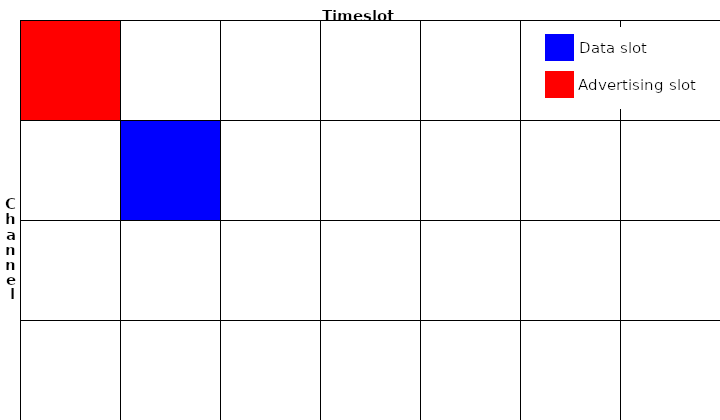
\includegraphics[width=.4\textwidth,keepaspectratio]{tsch_schedule.png}
	\caption{TSCH Schedule as used in the range analysis experiments}
	\label{fig:6tischStack}
\end{figure}


\subsubsection{Network stack}
\label{section:netstack}

For these experiments, most of the default Contiki-NG network stack has been disabled. We're interested in the performance of TSCH, so our experiments interact directly with the MAC layer. To facilitate this, Contiki-NG is built with the following Makefile variables set: 

\begin{itemize}
\item MAKE\_MAC=MAKE\_MAC\_TSCH
\item MAKE\_NET=MAKE\_NET\_NULLNET
\item MAKE\_ROUTING=MAKE\_ROUTING\_NULLROUTING
\end{itemize}

MAKE\_MAC\_TSCH tells the Make system to build the TSCH MAC layer, MAKE\_NET\_NULLNET essentially disables the network layer, MAKE\_ROUTING\_NULLROUTING does the same for routing functionality. 

\subsubsection{Preprocessor definitions}

The following values are defined in the preprocessor (some through Makefile, others through header definitions) in order to configure the behavior we want. Each parameter is briefly explained below.

\label{section:preprocessdef}
\begin{itemize}
\item $ENERGEST_CONF_ON=1$: Enable the energest package to allow analysis of power use. 
\item $TSCH_SCHEDULE_CONF_WITH_6TISCH_MINIMAL=0$: Disable creation of a default TSCH schedule. Instead we create our own, as described in section \ref{section:tschschedule}.
\item $LLSEC802154_CONF_ENABLED=0$: Disable Link Layer security.
\item $TSCH_CONF_JOIN_SECURED_ONLY=0$: Allow TSCH to join unsecured networks.
\item $TSCH_CONF_AUTOSTART=0$: Allow the program to start TSCH manually (using the NETSTACK\_MAC.on() function), rather than starting it immediately when the node powers on.
\end{itemize}


\subsection{Experiments}

Over the course of a minute, 60 packets are sent from the leaf node to the coordinator (root) node in each configuration. The configuration parameters being varied are the transmit power and the distance between the nodes, as discussed previously. 

The configurations are kept as close to identical as possible between various experimentation runs. The node positions at each distance were marked, to ensure they were positioned as reliably as possible. Between experiments where the tx power is changed, the tx power setting is the change in the code. 

A total of 12 runs were done - 3 different TX power values, tested at 4 different distances. 

In order to properly analyse the range capabilities, we must first define a test structure that will be repeated at each range. The test in this case is sending 120 packets (1 per second, 52 data bytes each) over a specified range (varying between 1 and 100 meters) so we can show the performance characteristics of TSCH as the distance between nodes varies. The data payload size was chosen out of convenience, as each packet carries metrics from the sender and they happened to be 52 bytes in size. Varying this packet size will result in different performance metrics and so must be addressed \ref{section:futurework}. 

Due to time constraints, combined with other obligations, the full scope of the experiments in this section has not yet been carried out. A brief comparison is made (showing the methodology) between nodes with 1 meter seperation and nodes with 5 meters seperation. Further work must be done to complete this analysis \ref{section:futurework}.

As of now, though, we can show that the TSCH functionality is essentially unchanged when we're looking at 1 vs 5 meters seperation between the two nodes. The power requirements are within margin of error, there is no significant packet loss in either case. The longer distance has a slightly higher latency (potentially caused by more retransmissions, we'll need to look at this \ref{section:futurework}).

For this analysis, we disabled the 6TiSCH stack (using only the TSCH mac layer) and ensured no security was enabled. No further changes to the Contiki-NG network stack were required. 

\subsection{Results}

\begin{figure}[]
	\centering
	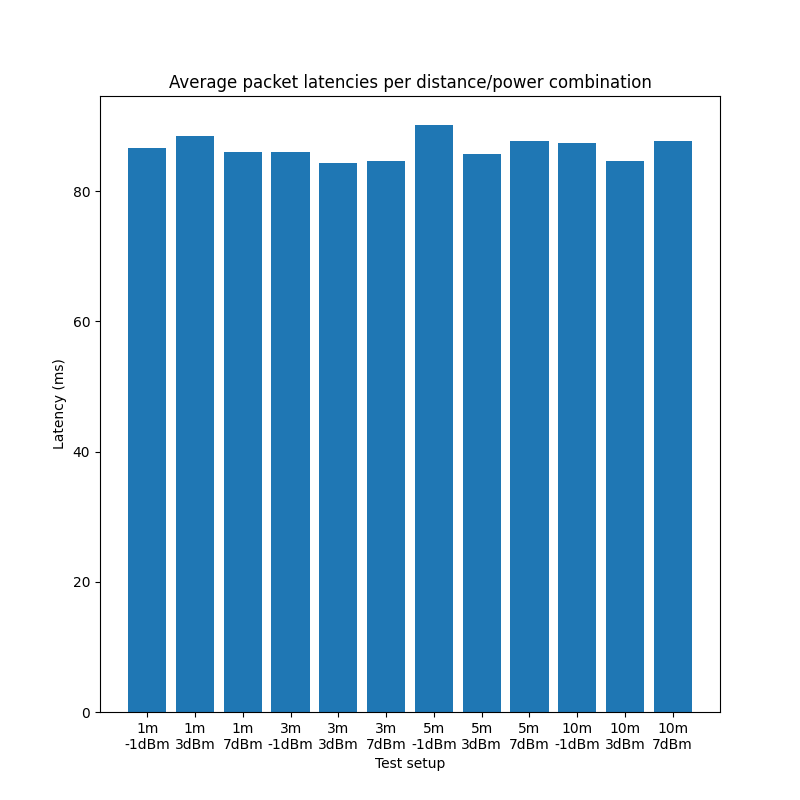
\includegraphics[width=.5\textwidth,keepaspectratio]{average_latencies.png}
	\caption{The average packet latencies for each distance/power combination}
	\label{fig:averagelatencies}
\end{figure}
\begin{figure}[]
	\centering
	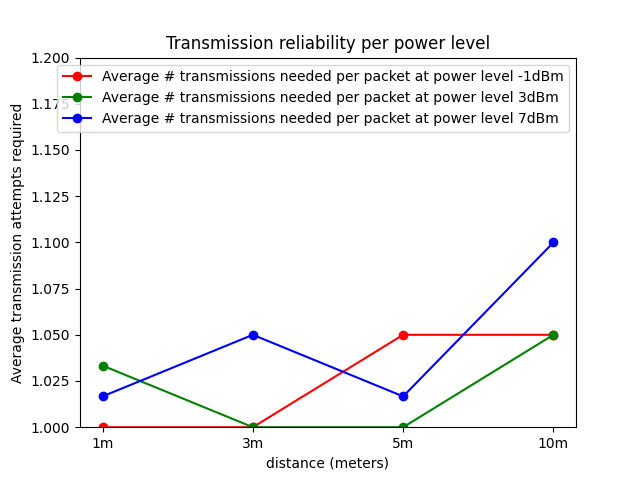
\includegraphics[width=.5\textwidth,keepaspectratio]{transmission_reliability.png}
	\caption{Overview of amount of transmission attempts are made on average to send a single packet}
	\label{fig:txattempts}
\end{figure}

In our current test scenario, there is no meaningful difference between the various power levels when it comes to transmission reliability. The amount of transmission attempts that must be made per packet are essentially identical (and almost equal to 1) for all tested scenario's. 

Another observation we can make, which is influenced by the transmission reliability, is the packet latency. In figure \ref{fig:averagelatencies}, the latencies are shown, averaged over the experiment run, per tested scenario. 

The latencies shown in figure \ref{fig:averagelatencies} are grouped very closely together, just over 80 milliseconds. Since the default TSCH slot length is 10 milliseconds, and the slot frame has 7 slots, it takes just over the duration of a slotframe for a packet to go from being queued in the leaf node to arriving at the root (give or take clock drift since the last TSCH time synchronization). This seems a little high, given the limited amount of traffic being generated. 


\begin{figure}[]
	\centering
	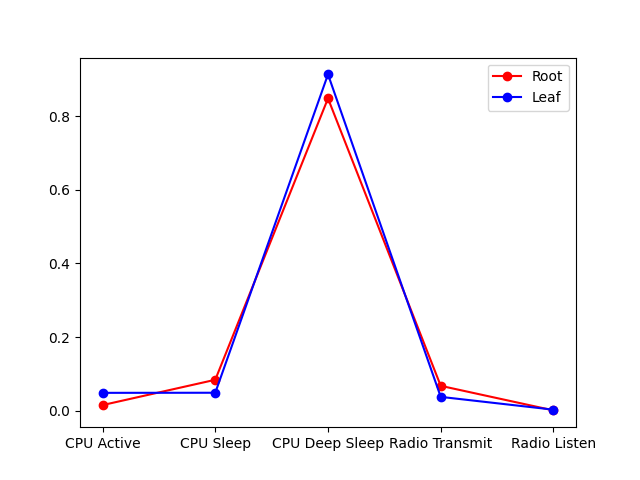
\includegraphics[width=.5\textwidth,keepaspectratio]{powerstates_10m.png}
	\caption{The power states for the nodes when 10 meters apart}
	\label{fig:power10m}
\end{figure}
\begin{figure}[]
	\centering
	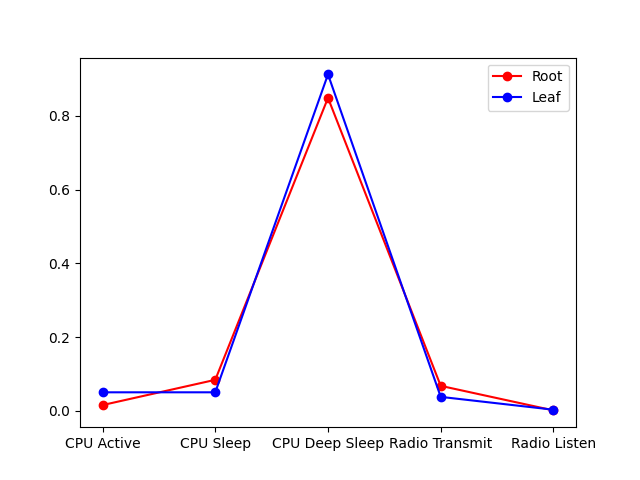
\includegraphics[width=.5\textwidth,keepaspectratio]{powerstates_1m.png}
	\caption{The power states for the nodes when 1 meter apart}
	\label{fig:power1m}
\end{figure}

The power results, as the latency and delivery results, are incredibly similar. This is trivially clear when comparing figures \ref{fig:power1m} and \ref{fig:power10m} - they are nearly identical. 

Using the results from profiling the device (as in \ref{tab:CurrentConsumption}), and the Energest results we've obtained, we can compute the amount of power that is needed for each device. The leaf, overall, used approximately 3.4 J. The root used approximately 4.1 J.

With a total data size of 360 kilobits (12 tests * 60 packets * 64 bytes per packet * 8 bits per byte / 1024 bits per kilobit), that corresponds to roughly $9.6 \frac{mJ}{kbit}$ for the leaf and $11.5 \frac{mJ}{kbit}$ for the root.


\subsection{Conclusion}

The tests we ran do not offer a clear insight to the performance of TSCH in various scenarios. The different scenarios appear too close together to distinguish meaningful differences. Due to the inherent noisiness of the wireless medium, the tests should be expanded to be able to clearly spot a pattern. The duration should be extended and the difference between the values under test should increase. This way, if there is a pattern, it is less likely that a difference in noise in the medium will cause the test results to be essentially indistinguishable. 

\section{Future Work}

\subsubsection{varied packet size}
In this study, we've only looked at the performance characteristics of the network at various distances for packets carrying 64 bytes of data payload. An interesting follow-up might be the analysis of how the results change when the packet size is varied as well. A sensor network doing less complex measurements could definitely get by with smaller packets, for example, which presumably makes transmitting and receiving them simpler (does allowing lower TX power for the same delivery performance). 

\subsubsection{individually varied TX power}
We've only considered the case where TX power is varied on both nodes. A potentially interesting follow-up to this is to consider the impact varying the parameter on one of the nodes has. This would clarify if, in order to ensure satisfactory network performance, TX power must be increased for all nodes or only for some. Our results have shown that larger TX power results in fewer retransmission (at the cost of increased power use per transmission), but we've not studied the trade-off in more detail.

\begin{thebibliography}{00}
\bibitem{contiki-NGWiki} Adam Dunkels, \url {https://github.com/contiki-ng/contiki-ng/wiki}
\bibitem{6tischDef} X. Vilajosana, T. Watteyne, T. Chang, M. Vučinić, S. Duquennoy and P. Thubert, "IETF 6TiSCH: A Tutorial," in IEEE Communications Surveys \& Tutorials, vol. 22, no. 1, pp. 595-615, Firstquarter 2020, doi: 10.1109/COMST.2019.2939407.
\bibitem{TimeCritical6tisch} Karaagac, Abdulkadir \& Haxhibeqiri, Jetmir \& Moerman, Ingrid \& Hoebeke, Jeroen. (2018). Time-critical communication in 6TiSCH networks. 161-166. 10.1109/WCNCW.2018.8368987. 
\bibitem{EnergyConsumption} Sabovic, Adnan \& Delgado, Carmen \& Bauwens, Jan \& De Poorter, Eli \& Famaey, Jeroen. (2019). Accurate Online Energy Consumption Estimation of IoT Devices Using Energest. 363-373. 10.1007/978-3-030-33506-9\_32. 
\bibitem{ThroughputEvaluation} Lee, S. B., Kim, E. J., \& Lim, Y. (2018). Contiki-NG-based IEEE 802.15. 4 TSCH Throughput Evaluation. In Proceedings of the Korean Institute of Information and Commucation Sciences Conference (pp. 577-578). The Korea Institute of Information and Commucation Engineering.
\bibitem{TSCHExperimentEval} García Algora, Carlos \& Alfonso Reguera, Vitalio. (2018). Experimental evaluation of IEEE 802.15.4 TSCH on a 6TiSCH network. 39. 70-78.
\bibitem{AccurateEnergyTSCH} Accurate Energy Consumption Modeling of IEEE 802.15.4e TSCH Using Dual-BandOpenMote Hardware
Glenn Daneels, Esteban Municio, Bruno Van de Velde, Glenn Ergeerts, Maarten Weyn, Steven Latré, \& Jeroen Famaey

\end{thebibliography}

\end{document}
